\documentclass[11pt,a4paper]{article}

\usepackage[T1]{fontenc}
\usepackage{mathpazo}
\usepackage[margin=2.6cm]{geometry}
\usepackage{microtype}
\usepackage{amsmath,amssymb}
\usepackage{graphicx}
\usepackage{booktabs}
\usepackage{xcolor}
\usepackage[font=small,labelfont=bf]{caption}
\usepackage[colorlinks=true,linkcolor=blue!50!black,citecolor=blue!50!black,urlcolor=blue!50!black]{hyperref}

\graphicspath{{../figures/}}
% Generated by experiments/run_experiments.py -- do not edit by hand.
\newcommand{\CallPrice}{4.23}
\newcommand{\InitDelta}{0.540}
\newcommand{\Mmain}{20{,}000}
\newcommand{\Msweep}{10{,}000}
\newcommand{\StdWeekly}{0.96}
\newcommand{\MeanWeekly}{-0.009}
\newcommand{\StdDaily}{0.44}
\newcommand{\MeanDaily}{-0.001}
\newcommand{\StdIntraday}{0.22}
\newcommand{\MeanIntraday}{+0.001}
\newcommand{\Slope}{-0.489}
\newcommand{\DKmaxRelErr}{8}
\newcommand{\DriftBiasDaily}{0.028}
\newcommand{\DriftBiasFine}{0.0007}
\newcommand{\kpct}{0.4}
\newcommand{\BestN}{64}
\newcommand{\BestRMS}{0.79}
\newcommand{\CostLossMaxN}{2.13}
\newcommand{\MaxNtc}{1024}
\newcommand{\StdMinTc}{0.42}
\newcommand{\StdMinTcN}{128}
\newcommand{\SetupCost}{0.108}
\newcommand{\LelandMeanMin}{-0.111}
\newcommand{\LelandMeanMax}{-0.093}
\newcommand{\LelandStdMaxN}{0.13}
\newcommand{\BSStdMaxN}{0.78}
\newcommand{\LelandSigDaily}{22.4}
\newcommand{\LelandPriceDaily}{4.71}
\newcommand{\SigImp}{20}
\newcommand{\SigReal}{15}
\newcommand{\PriceGap}{0.997}
\newcommand{\Nfine}{1000}
\newcommand{\CorrFine}{0.978}
\newcommand{\ResidStdFine}{0.070}
\newcommand{\ImpMean}{0.988}
\newcommand{\ImpStd}{0.334}
\newcommand{\RealMean}{0.997}
\newcommand{\RealStd}{0.083}
\newcommand{\ImpLossProb}{0.0}
\newcommand{\ImpMin}{0.16}
\newcommand{\ImpMax}{1.92}
\newcommand{\WrongVolRows}{16 & 0.986 & 0.703 & 0.992 & 0.627 \\
64 & 0.987 & 0.447 & 0.994 & 0.318 \\
256 & 0.987 & 0.362 & 0.999 & 0.164 \\
1024 & 0.995 & 0.335 & 0.997 & 0.083 \\}


% Edit this line once the GitHub repository exists.
\newcommand{\repourl}{https://github.com/USERNAME/delta-hedging}

\newcommand{\E}{\mathbb{E}}
\newcommand{\dd}{\mathrm{d}}
\newcommand{\PnL}{\text{P\&L}}

\title{\textbf{Delta Hedging in Discrete Time:\\[2pt]
\large Rebalancing Error, Transaction Costs and Volatility Misspecification}}
\author{Gabriel Baraban\\[2pt]
\small École Polytechnique, Bachelor of Science (Mathematics \& Economics)}
\date{October 2026}

\begin{document}
\maketitle

\begin{abstract}
\noindent
In the Black--Scholes model a European call can be replicated exactly by trading continuously in the underlying stock. This note studies, by Monte Carlo simulation, what remains of this result under three realistic departures: the hedge is rebalanced at finitely many dates, every trade incurs a proportional cost, and the volatility used to hedge differs from the one realised by the market. For each case I derive the leading-order behaviour of the hedger's profit and loss with an elementary Itô--Taylor argument and compare it with simulations. The rebalancing error decays like $N^{-1/2}$ in the number $N$ of rebalancing dates; with costs, the expected loss grows like $N^{1/2}$, which creates an optimal rebalancing frequency, and Leland's adjusted volatility removes almost all of the cost bias; with a misspecified volatility, the profit is driven by the gamma-weighted gap between implied and realised variance, which I verify path by path. All code is available at \url{\repourl}.
\end{abstract}

\section{Introduction}

The Black--Scholes price of an option is the initial cost of a self-financing portfolio that replicates its payoff \cite{BlackScholes1973}. Replication requires trading continuously, in a frictionless market, with knowledge of the true volatility. None of these holds in practice, so a trader who sells an option at its Black--Scholes price and hedges it is exposed to a residual profit and loss (\PnL).

This note quantifies that residual in a controlled setting. The stock follows a geometric Brownian motion; a trader sells a three-month at-the-money call and delta-hedges it. Three questions are studied, one per section:
\begin{enumerate}
  \item How large is the hedging error when the hedge is rebalanced only $N$ times? (Section~\ref{sec:discrete})
  \item How do proportional transaction costs change the picture, and can they be priced in? (Section~\ref{sec:costs})
  \item What happens when the trader hedges with a volatility different from the realised one? (Section~\ref{sec:wrongvol})
\end{enumerate}
The answers are classical \cite{Leland1985,DermanKamal1999,ElKarouiEtAl1998,AhmadWilmott2005,BouchardChassagneux2016}; the purpose here is to re-derive the mechanisms in a unified way and to check each prediction numerically.

\section{Setting}\label{sec:setting}

\paragraph{Model.} Under the real-world probability the stock satisfies
\begin{equation}\label{eq:gbm}
  \dd S_t = \mu S_t\,\dd t + \sigma S_t\,\dd W_t ,
\end{equation}
and cash earns the constant rate $r$. The Black--Scholes price of a call with strike $K$ and maturity $T$ is
\[
  C(t,S) = S\,\Phi(d_1) - K e^{-r\tau}\Phi(d_2),\qquad
  d_{1,2} = \frac{\ln(S/K) + (r\pm\tfrac12\sigma^2)\tau}{\sigma\sqrt\tau},\qquad \tau = T-t,
\]
with delta $\Delta = \partial_S C = \Phi(d_1)$ and gamma $\Gamma = \partial_{SS} C = \varphi(d_1)/(S\sigma\sqrt\tau)$. The price solves the Black--Scholes equation
\begin{equation}\label{eq:bspde}
  \partial_t C + \tfrac12\sigma^2 S^2\,\Gamma + rS\,\Delta - rC = 0 .
\end{equation}
Throughout, $S_0 = K = 100$, $T = 0.25$, $r = 2\%$, $\mu = 8\%$ and $\sigma = 20\%$, so that $C(0,S_0) = \CallPrice$.

\paragraph{Hedging strategy.} The trader sells the call at time $0$ for $C(0,S_0)$, buys $\Delta_0$ shares and keeps the rest in cash. At the dates $t_i = iT/N$, $i = 1,\dots,N-1$, the position is adjusted to $\Delta_{t_i}$ shares, the trade being financed from cash; no money is added or withdrawn. At maturity the trader pays $(S_T-K)^+$. The terminal \PnL\ is
\[
  \PnL = B_T + \Delta_{t_{N-1}} S_T - (S_T - K)^+ ,
\]
where $B_T$ is the cash account. Under continuous rebalancing in the model \eqref{eq:gbm}, $\PnL = 0$ almost surely.

\paragraph{Simulation.} Paths are simulated exactly on the grid,
$S_{t_{i+1}} = S_{t_i}\exp\big((\mu - \tfrac12\sigma^2)\Delta t + \sigma\sqrt{\Delta t}\,Z_i\big)$ with $Z_i$ i.i.d.\ standard normal and $\Delta t = T/N$, so the only approximation is the discreteness of the hedge. Results use $\Mmain$ paths for the main figures and $\Msweep$ paths per point in the parameter sweeps.

\section{Discrete rebalancing}\label{sec:discrete}

\paragraph{Local error.} Consider one period $[t_i, t_{i+1}]$ and write $\delta S = S_{t_{i+1}} - S_{t_i}$. To second order, the option moves by $\partial_t C\,\Delta t + \Delta\,\delta S + \tfrac12\Gamma\,\delta S^2$, the shares by $\Delta\,\delta S$, and the cash, which equals $C - \Delta S$ when the portfolio is balanced, earns $r(C - \Delta S)\Delta t$. Using \eqref{eq:bspde} to eliminate $\partial_t C$, the change in the hedged position of the option seller is
\begin{equation}\label{eq:localerror}
  \varepsilon_i \approx \tfrac12\,\Gamma_{t_i} S_{t_i}^2\left(\sigma^2\Delta t - \Big(\frac{\delta S}{S_{t_i}}\Big)^2\right)
  \approx \tfrac12\,\Gamma_{t_i} S_{t_i}^2\,\sigma^2\Delta t\,\big(1 - Z_i^2\big).
\end{equation}
The delta terms cancel exactly: this is why the drift $\mu$ plays no role. What is left is a convexity term, of zero mean, because $\E[Z_i^2] = 1$, and of variance $\tfrac12(\Gamma S^2\sigma^2\Delta t)^2$, because $\operatorname{Var}(Z^2) = 2$.

\paragraph{Global error.} The local errors are uncorrelated, so their variances add:
\[
  \operatorname{Var}(\PnL) \approx \tfrac12\sum_{i} \E\big[(\Gamma_{t_i}S_{t_i}^2\sigma^2)^2\big]\Delta t^2
  \approx \frac{T}{2N}\int_0^T \E\big[(\Gamma_t S_t^2\sigma^2)^2\big]\,\dd t .
\]
The standard deviation of the \PnL\ therefore decays like $N^{-1/2}$. For an at-the-money option, Derman and Kamal \cite{DermanKamal1999} obtain the explicit approximation
\begin{equation}\label{eq:dk}
  \operatorname{Std}(\PnL) \approx \sqrt{\frac{\pi}{4}}\;\frac{\sigma\,\mathcal V}{\sqrt N},\qquad \mathcal V = \partial_\sigma C(0,S_0).
\end{equation}

\paragraph{Results.} Figure~\ref{fig:hist} shows the \PnL\ distribution for weekly ($N=12$), daily ($N=63$) and four-times-daily ($N=252$) rebalancing. The distributions are centred at zero (means $\MeanWeekly$, $\MeanDaily$ and $\MeanIntraday$) with standard deviations $\StdWeekly$, $\StdDaily$ and $\StdIntraday$: multiplying $N$ by four roughly halves the error. Figure~\ref{fig:conv} confirms the rate: the fitted log--log slope is $\Slope$, against $-0.5$ in theory, and \eqref{eq:dk} is within $\DKmaxRelErr\%$ of the simulation over the whole range.

\begin{figure}[t]
  \centering
  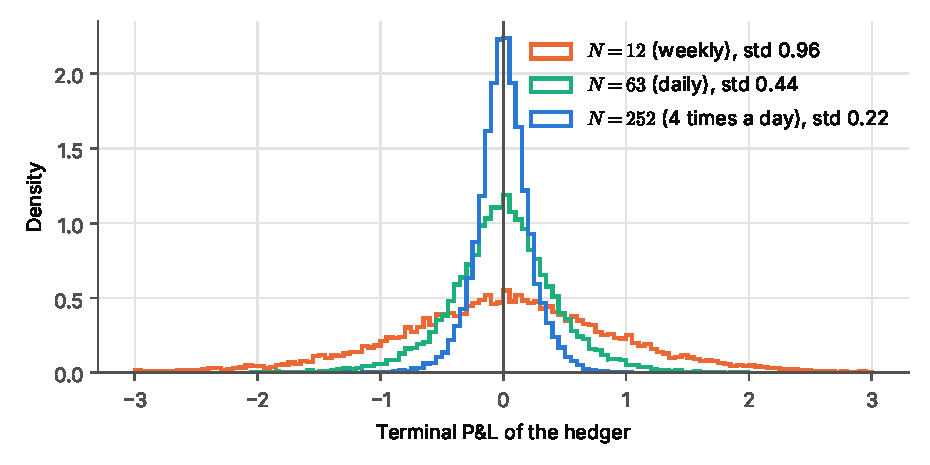
\includegraphics[width=0.82\textwidth]{fig1_pnl_hist.pdf}
  \caption{Distribution of the terminal \PnL\ of a delta-hedged short call for three rebalancing frequencies. The option is worth $\CallPrice$.}
  \label{fig:hist}
\end{figure}

\begin{figure}[t]
  \centering
  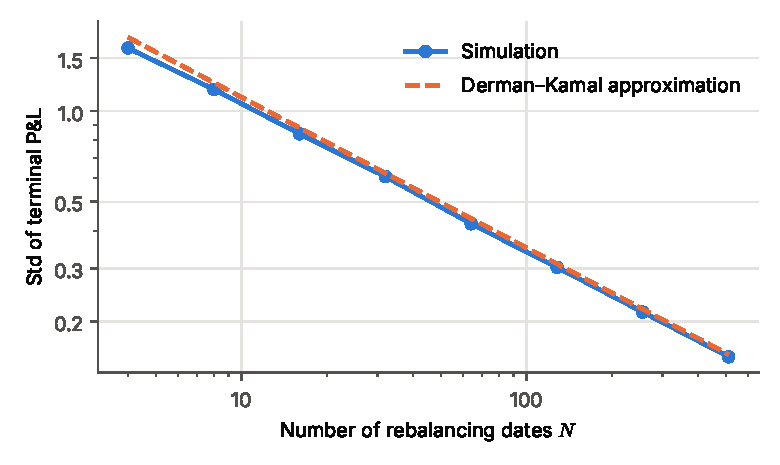
\includegraphics[width=0.68\textwidth]{fig2_convergence.pdf}
  \caption{Standard deviation of the \PnL\ against $N$ (log--log scale), with the Derman--Kamal approximation \eqref{eq:dk}.}
  \label{fig:conv}
\end{figure}

\paragraph{Role of the drift.} The cancellation in \eqref{eq:localerror} only holds to leading order. Hedging under drifts of $-20\%$ and $+40\%$, the mean \PnL\ moves by at most $\DriftBiasDaily$ with daily rebalancing and by at most $\DriftBiasFine$ with $N = 1000$: the drift affects the hedge only through discretisation effects, which vanish as $N\to\infty$.

\section{Transaction costs}\label{sec:costs}

\paragraph{Cost model.} Each trade of $n$ shares at price $S$ now costs $\tfrac{k}{2}|n|S$, where $k$ is the round-trip proportional cost; I take $k = \kpct\%$. All rebalancing trades, including the initial purchase of $\Delta_0$ shares, are charged.

\paragraph{Scaling of the cost.} Over one period the hedge ratio changes by $\delta\Delta \approx \Gamma\,\delta S \approx \Gamma S\sigma\sqrt{\Delta t}\,Z$. Since $\E|Z| = \sqrt{2/\pi}$, the expected cost of one rebalance is
\begin{equation}\label{eq:stepcost}
  \E[\text{cost}_i] \approx \frac{k}{2}\sqrt{\frac{2}{\pi}}\;\sigma\,\Gamma_{t_i} S_{t_i}^2\sqrt{\Delta t},
\end{equation}
and the total expected cost, a sum of $N$ such terms, grows like $N\sqrt{\Delta t} \propto \sqrt N$. Frequent rebalancing reduces the hedging error of Section~\ref{sec:discrete} but increases the bill: costs grow like $\sqrt N$ while the error shrinks like $1/\sqrt N$.

\paragraph{Results.} Figure~\ref{fig:costs} shows the trade-off. The expected loss increases steadily with $N$ and reaches $\CostLossMaxN$, half the option's value, at $N = \MaxNtc$. The standard deviation is no longer monotone: it falls to $\StdMinTc$ at $N = \StdMinTcN$ and then rises again, because the random amount of costs paid becomes itself a source of risk. The root-mean-square \PnL, which penalises both bias and risk, is minimised at $N = \BestN$, roughly daily rebalancing. Exact replication is no longer possible, and selling at the Black--Scholes price is a losing strategy on average.

\begin{figure}[t]
  \centering
  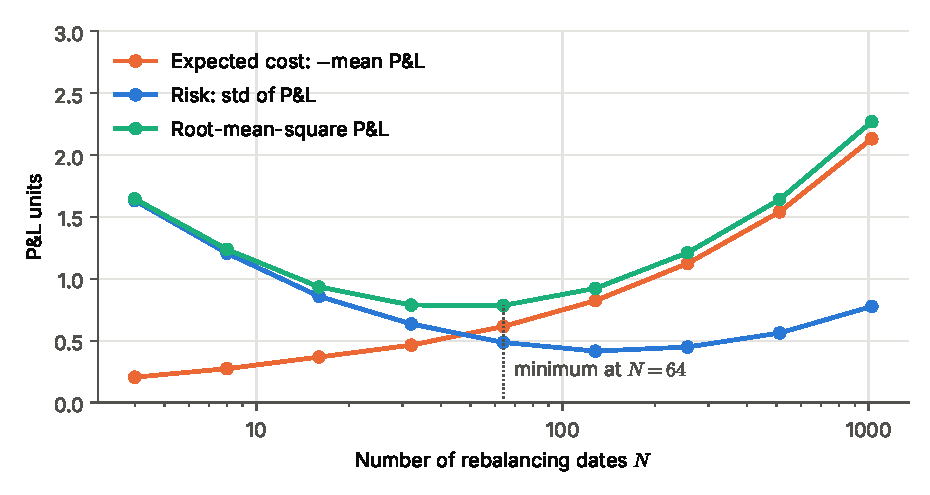
\includegraphics[width=0.82\textwidth]{fig3_costs.pdf}
  \caption{Hedging with transaction costs ($k = \kpct\%$ round trip): expected cost, risk, and root-mean-square \PnL\ against the number of rebalancing dates.}
  \label{fig:costs}
\end{figure}

\paragraph{Leland's correction.} Equation \eqref{eq:stepcost} has the same form as the convexity term in \eqref{eq:localerror}: both are proportional to $\Gamma S^2$. The cost can therefore be absorbed into an enlarged variance. Requiring the extra convexity premium $\tfrac12\Gamma S^2(\hat\sigma^2 - \sigma^2)\Delta t$ to pay for the expected cost \eqref{eq:stepcost} gives Leland's volatility \cite{Leland1985}
\begin{equation}\label{eq:leland}
  \hat\sigma^2 = \sigma^2\left(1 + \sqrt{\frac{2}{\pi}}\;\frac{k}{\sigma\sqrt{\Delta t}}\right).
\end{equation}
The trader sells the option at the Black--Scholes price computed with $\hat\sigma$ and hedges with the corresponding delta. For daily rebalancing, $\hat\sigma = \LelandSigDaily\%$ and the option is sold for $\LelandPriceDaily$ instead of $\CallPrice$.

Figure~\ref{fig:leland} compares the two strategies. With Leland's volatility the mean \PnL\ stays between $\LelandMeanMin$ and $\LelandMeanMax$ for every $N$. This residual is the cost of buying the initial hedge, $\tfrac{k}{2}\Delta_0 S_0 = \SetupCost$, a one-off trade that \eqref{eq:leland}, built from rebalancing costs, does not price. The risk also keeps decreasing with $N$, to $\LelandStdMaxN$ at $N = \MaxNtc$ against $\BSStdMaxN$ for the Black--Scholes hedge. The approximation behind \eqref{eq:leland} requires $k/(\sigma\sqrt{\Delta t})$ to remain moderate; as $\Delta t\to 0$ with $k$ fixed, $\hat\sigma$ explodes, and it is known that perfect hedging under proportional costs is impossible in that limit.

\begin{figure}[t]
  \centering
  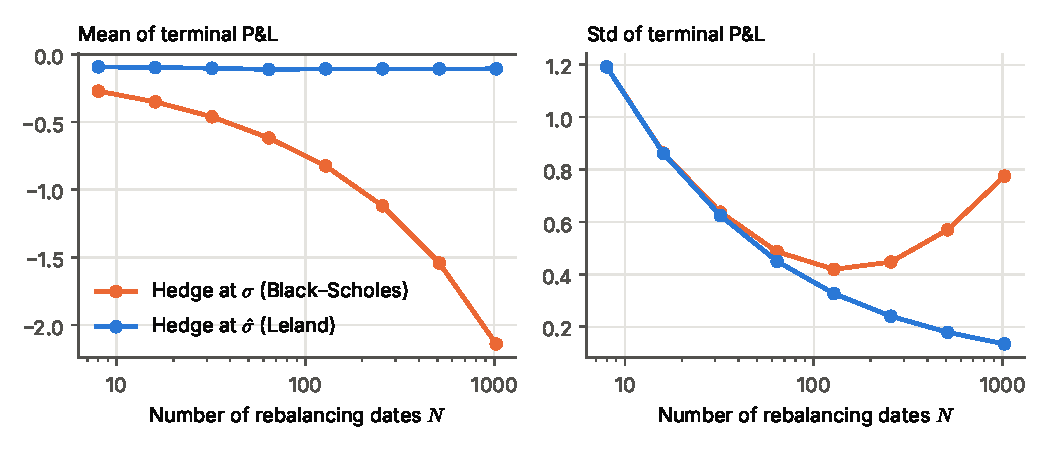
\includegraphics[width=0.95\textwidth]{fig4_leland.pdf}
  \caption{Mean (left) and standard deviation (right) of the \PnL\ under transaction costs, when pricing and hedging with the true volatility $\sigma$ or with Leland's volatility $\hat\sigma$.}
  \label{fig:leland}
\end{figure}

\section{Hedging with the wrong volatility}\label{sec:wrongvol}

In practice the volatility is not observed. Options trade at an \emph{implied} volatility $\Sigma$, while the stock realises some volatility $\sigma$ that is only known after the fact. Here the stock realises $\sigma = \SigReal\%$ while the option is sold at $\Sigma = \SigImp\%$. Costs are set to zero.

\paragraph{Hedging at the implied volatility.} Let $C^\Sigma$, $\Delta^\Sigma$, $\Gamma^\Sigma$ denote the Black--Scholes quantities computed with $\Sigma$. Repeating the computation of Section~\ref{sec:discrete} in continuous time, but using the Black--Scholes equation \eqref{eq:bspde} at volatility $\Sigma$ while $S$ has quadratic variation $\sigma^2S^2\,\dd t$, Itô's formula gives for the seller's hedged position $\Pi$
\[
  \dd\Pi_t - r\Pi_t\,\dd t = \tfrac12\,\Gamma^\Sigma_t S_t^2\left(\Sigma^2 - \sigma^2\right)\dd t ,
\]
so that
\begin{equation}\label{eq:gammapnl}
  \PnL = \frac{\Sigma^2 - \sigma^2}{2}\int_0^T e^{r(T-t)}\,\Gamma^\Sigma_t S_t^2\,\dd t .
\end{equation}
This is the classical robustness formula of El Karoui, Jeanblanc-Picqué and Shreve \cite{ElKarouiEtAl1998}. Since $\Gamma > 0$ for a call, the seller makes money on \emph{every} path when the implied volatility exceeds the realised one, but the amount depends on the path: it is large when the stock stays close to the strike near maturity, where gamma is concentrated.

\paragraph{Hedging at the realised volatility.} Alternatively, the trader sells at $C^\Sigma$ but hedges with $\Delta^\sigma$. The hedge then replicates exactly a call priced at $\sigma$, and the trader keeps the price difference:
\begin{equation}\label{eq:lockedin}
  \PnL = e^{rT}\big(C^\Sigma(0,S_0) - C^\sigma(0,S_0)\big) = \PriceGap .
\end{equation}
The profit is deterministic, but the strategy requires knowing $\sigma$ in advance.

\paragraph{Results.} The left panel of Figure~\ref{fig:wrongvol} plots, path by path, the simulated \PnL\ of the implied-volatility hedge against the prediction \eqref{eq:gammapnl}, evaluated on the same path. With $N = \Nfine$ the correlation is $\CorrFine$, and the residual, which is the discrete-rebalancing error of Section~\ref{sec:discrete}, has standard deviation $\ResidStdFine$. The \PnL\ is positive on all $\Mmain$ paths, ranging from $\ImpMin$ to $\ImpMax$.

The right panel compares the two strategies. Both earn about the price gap on average ($\ImpMean$ and $\RealMean$, against $\PriceGap$ from \eqref{eq:lockedin}), but their risks differ: $\ImpStd$ for the implied hedge against $\RealStd$ for the realised one. Table~\ref{tab:wrongvol} shows that the second number tends to zero as $N$ grows, while the first levels off. Its randomness is not a discretisation artefact; it is intrinsic to \eqref{eq:gammapnl}.

\begin{figure}[t]
  \centering
  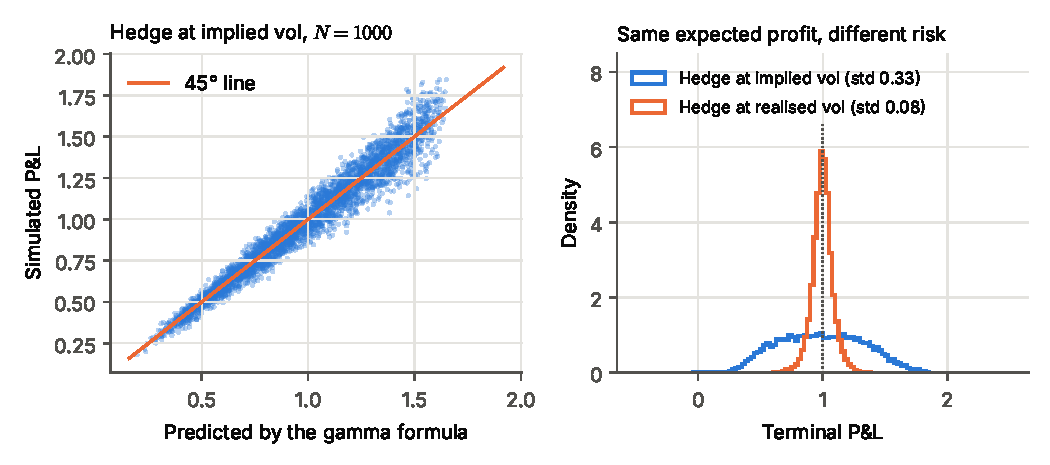
\includegraphics[width=0.95\textwidth]{fig5_wrong_vol.pdf}
  \caption{Option sold at implied volatility $\Sigma = \SigImp\%$, stock realising $\sigma = \SigReal\%$. Left: simulated \PnL\ of the implied-volatility hedge against formula \eqref{eq:gammapnl}, on 4{,}000 paths. Right: \PnL\ of the implied-volatility and realised-volatility hedges; the dotted line is the locked-in profit \eqref{eq:lockedin}.}
  \label{fig:wrongvol}
\end{figure}

\begin{table}[t]
  \centering
  \begin{tabular}{rcccc}
    \toprule
    & \multicolumn{2}{c}{Hedge at implied $\Sigma$} & \multicolumn{2}{c}{Hedge at realised $\sigma$} \\
    \cmidrule(lr){2-3}\cmidrule(lr){4-5}
    $N$ & mean & std & mean & std \\
    \midrule
    \WrongVolRows
    \bottomrule
  \end{tabular}
  \caption{\PnL\ of the two hedging strategies when $\Sigma = \SigImp\%$ and $\sigma = \SigReal\%$ ($\Msweep$ paths per row). Only the realised-volatility hedge converges to a deterministic profit.}
  \label{tab:wrongvol}
\end{table}

\section{Conclusion}

Each departure from the Black--Scholes assumptions leaves a residual whose leading-order behaviour follows from the same second-order expansion. Discrete rebalancing creates an error of order $N^{-1/2}$; proportional costs create a bias of order $N^{1/2}$, hence an optimal rebalancing frequency, and Leland's volatility prices this bias in almost entirely; a misspecified volatility creates a profit driven by the gamma-weighted gap between implied and realised variance. In every case the simulations agree with the leading-order formulas.

Two directions seem natural to pursue. First, Leland's correction is an approximation: with transaction costs, the exact superhedging price solves a \emph{nonlinear} pricing equation, which can be written as a backward stochastic differential equation (BSDE) \cite{BouchardChassagneux2016}. Solving such equations numerically, and comparing the result with Leland's formula, would make the analysis of Section~\ref{sec:costs} exact rather than asymptotic. Second, the hedging dates were fixed in advance; rebalancing only when the delta leaves a band around its target is a simple way to trade fewer shares for the same risk, and comparing it with calendar hedging would refine the trade-off of Figure~\ref{fig:costs}.

\paragraph{Reproducibility.} Every figure and every number in this note is produced by a single script, \texttt{experiments/run\_experiments.py}, which writes the numbers into the \LaTeX\ source. The code, with unit tests, is available at \url{\repourl}.

\begin{thebibliography}{9}
\small
\bibitem{AhmadWilmott2005}
R.~Ahmad and P.~Wilmott, \emph{Which free lunch would you like today, sir? Delta hedging, volatility arbitrage and optimal portfolios}, Wilmott Magazine, November 2005, 64--79.

\bibitem{BlackScholes1973}
F.~Black and M.~Scholes, \emph{The pricing of options and corporate liabilities}, Journal of Political Economy 81 (1973), 637--654.

\bibitem{BouchardChassagneux2016}
B.~Bouchard and J.-F.~Chassagneux, \emph{Fundamentals and Advanced Techniques in Derivatives Hedging}, Universitext, Springer, 2016.

\bibitem{DermanKamal1999}
E.~Derman and M.~Kamal, \emph{When you cannot hedge continuously: the corrections to Black--Scholes}, Risk 12 (1999), 82--85.

\bibitem{ElKarouiEtAl1998}
N.~El Karoui, M.~Jeanblanc-Picqué and S.~E.~Shreve, \emph{Robustness of the Black and Scholes formula}, Mathematical Finance 8 (1998), 93--126.

\bibitem{Leland1985}
H.~E.~Leland, \emph{Option pricing and replication with transactions costs}, Journal of Finance 40 (1985), 1283--1301.
\end{thebibliography}

\end{document}
